\section{Initial Results}
\label{section_result_initial_results}

This section presents our initial results,
aimed at replicating the findings from \citen{Arthur2023} to ensure the integrity of our implementation.
We tested our algorithm on 100 randomly generated 40x40 perfect mazes \cite{Naeem2021}, incrementing the number of agents from 1 to 40.
We evaluated:

\begin{itemize}
    \item Total steps taken by all agents.
    \item Steps taken by the pioneer (first agent to find the goal).
    \item Fraction of the maze explored.
    \item Fraction explored before the pioneer found the goal.
\end{itemize}

Figures \ref{fig_comparison_steps} and \ref{fig_comparison_fraction} show a side-by-side comparison of our results with those from \citen{Arthur2023}.

\begin{figure}[H]
\centering
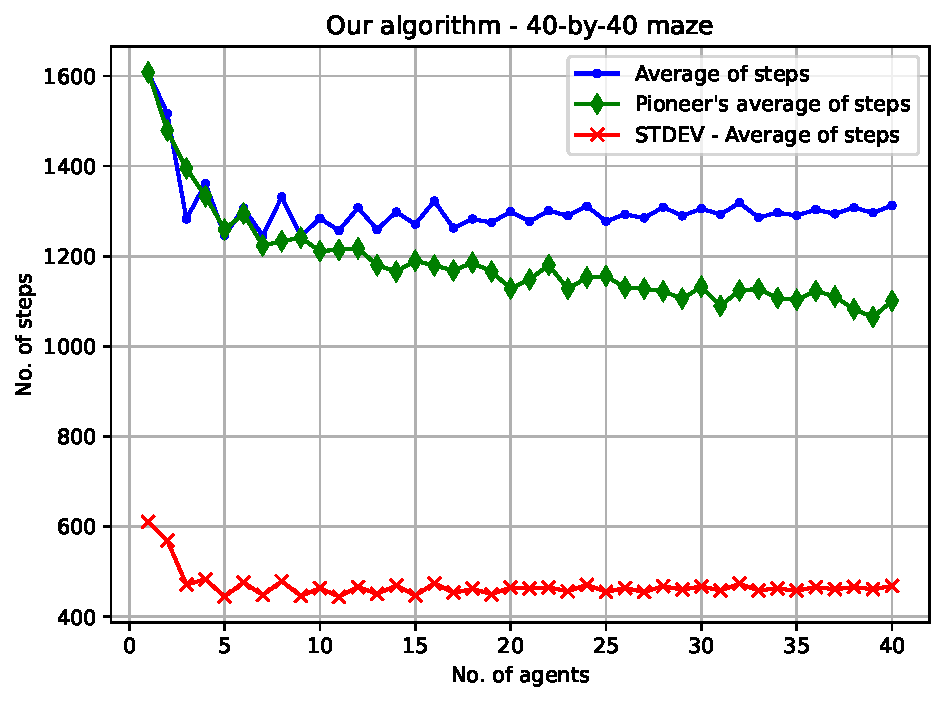
\includegraphics[height=5cm]{Cap3/arthur_40x40_steps.pdf}
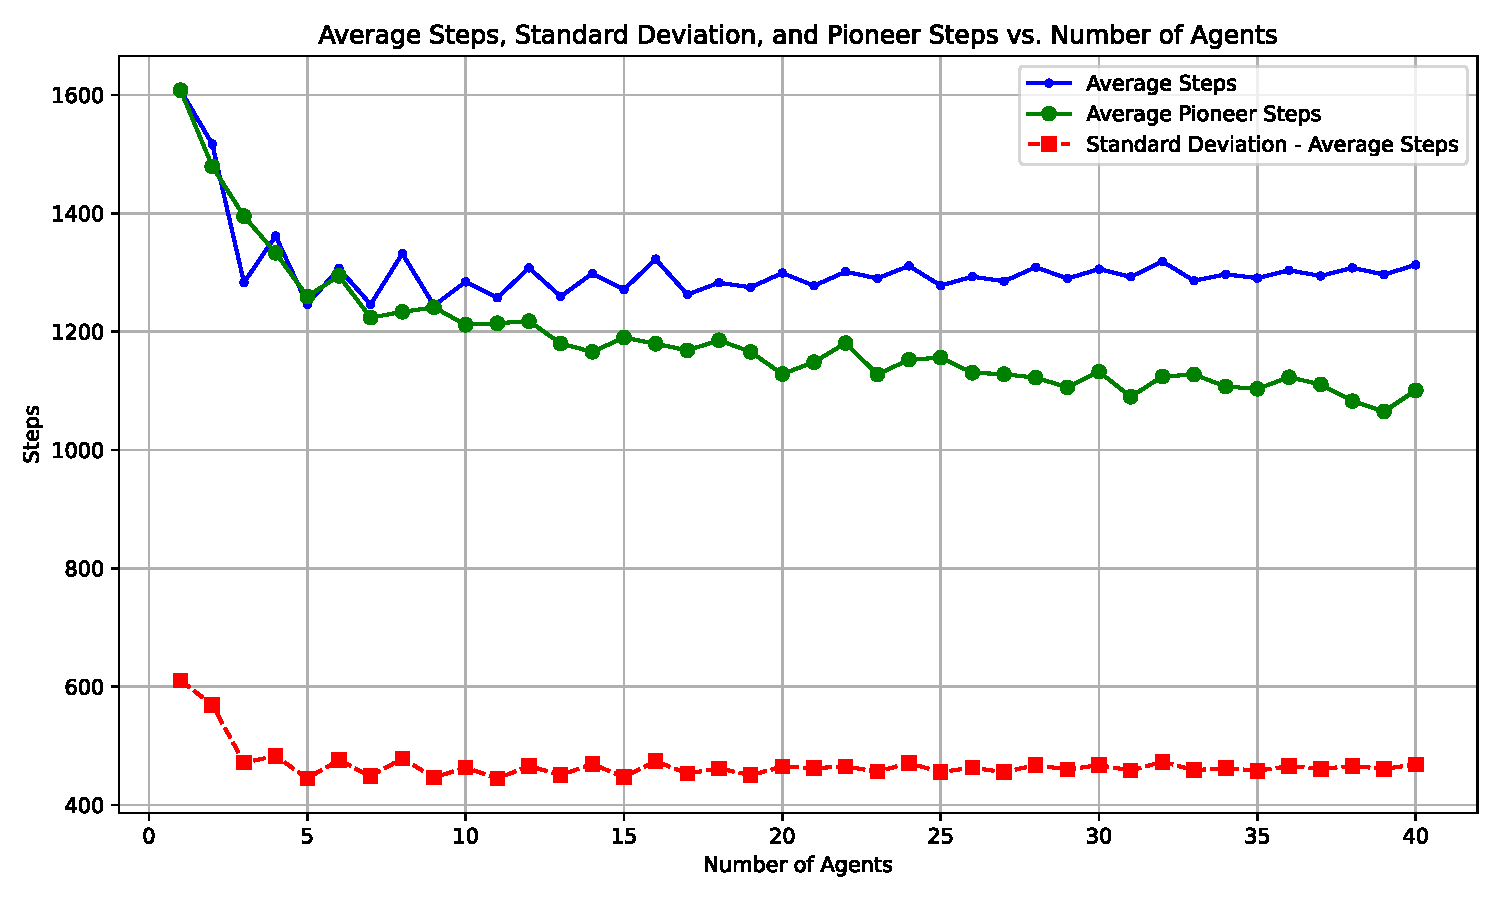
\includegraphics[height=5cm]{Cap3/self_steps_40x40.pdf}
\caption{Comparison of total steps: Left - Results from \citen{Arthur2023}; Right - Our results}
\label{fig_comparison_steps}
\end{figure}

\begin{figure}[H]
    \centering
    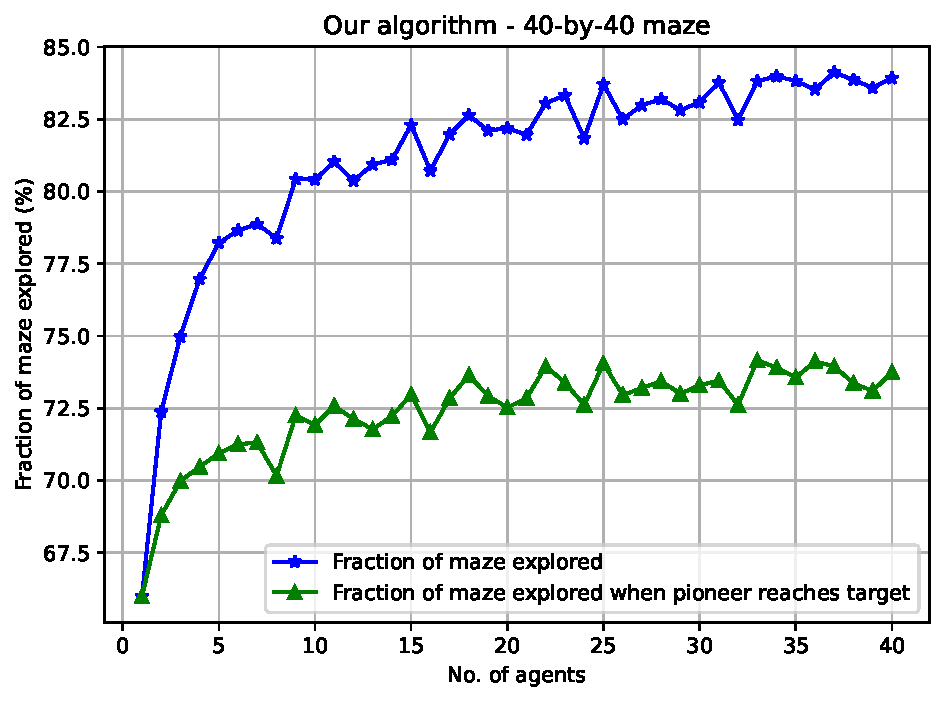
\includegraphics[height=5cm]{Cap3/arthur_40x40_fraction.pdf}
    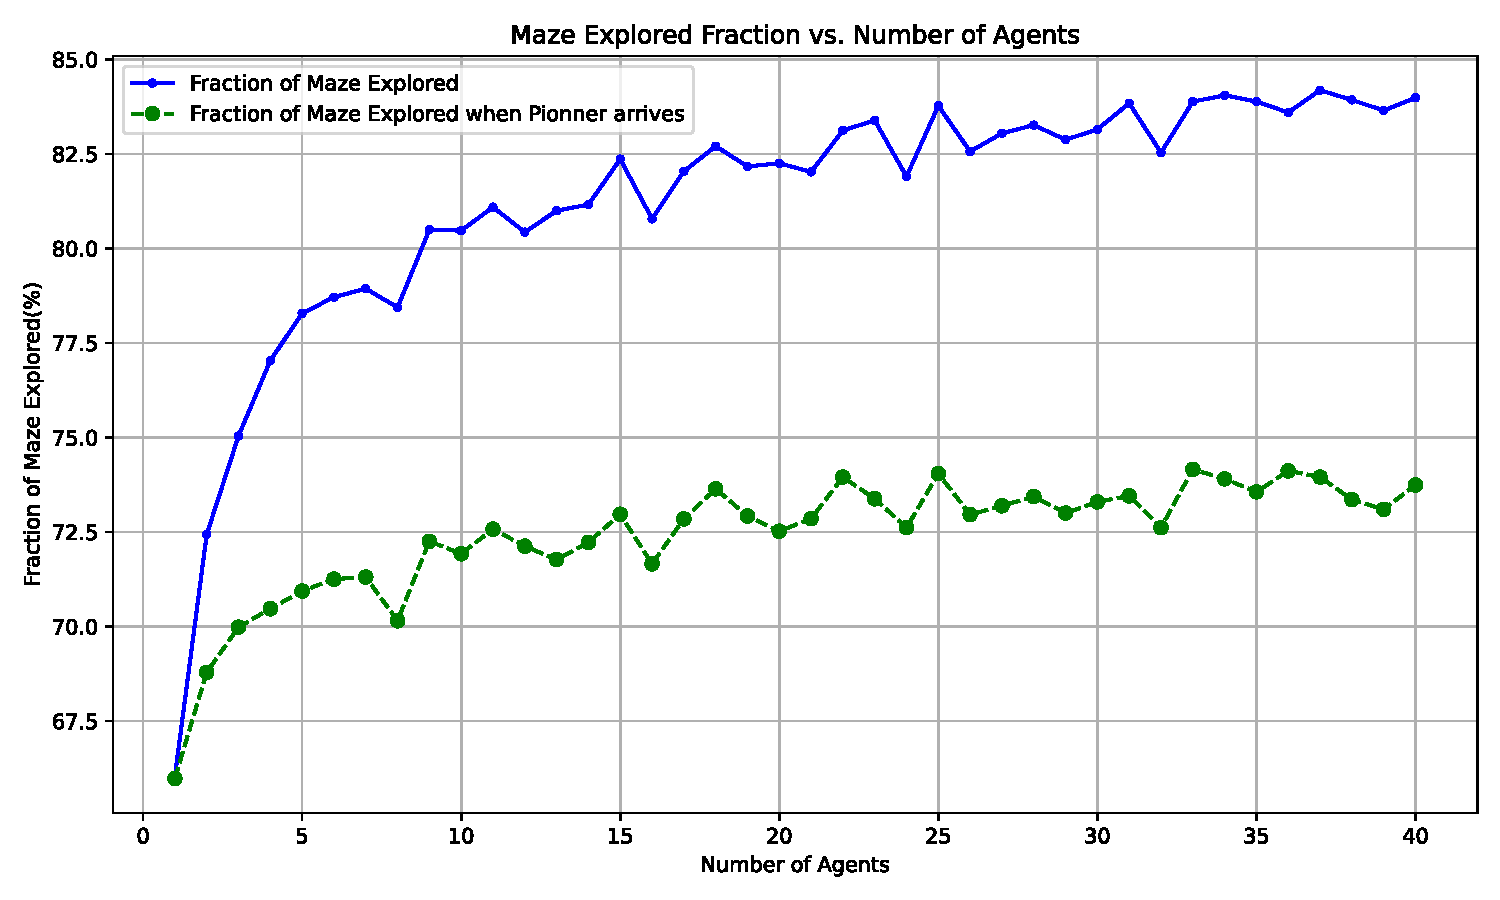
\includegraphics[height=5cm]{Cap3/self_fraction_40x40.pdf}
    \caption{Comparison of explored fraction: Left - Results from \citen{Arthur2023}; Right - Our results}
\label{fig_comparison_fraction}
\end{figure}

As evident from the figures, our results closely match the original findings,
demonstrating that our modifications have not altered the core functionality of the algorithm.

\section{Visualization Improvements}
\label{section_result_visualization}

Another significant improvement is the visualization capability for graphs.

To demonstrate this, we ran the algorithm on an imperfect maze, a cyclic graph, using three agents.
Below, we present the results: the overall exploration of the maze and the individual trees constructed by each agent.

\begin{figure}[H]
\centering
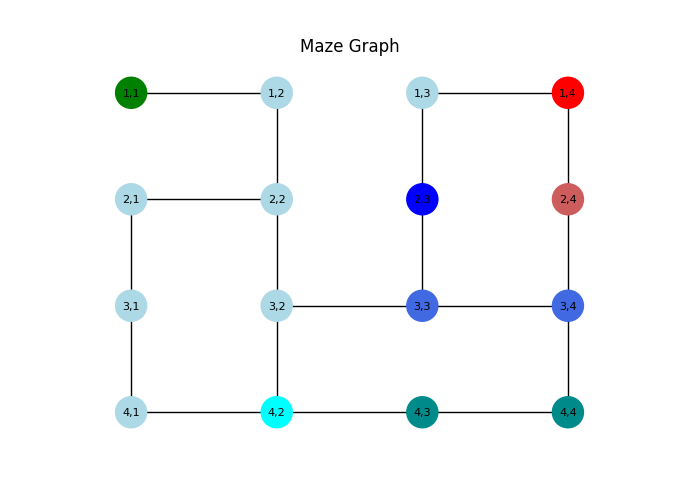
\includegraphics[width=0.5\textwidth]{Cap3/maze_imperfect_exploration.png}
\caption{Exploration of an imperfect maze(graph) by three agents.}
\label{fig_imperfect_maze_exploration}
\end{figure}
    
\begin{figure}[H]
\centering
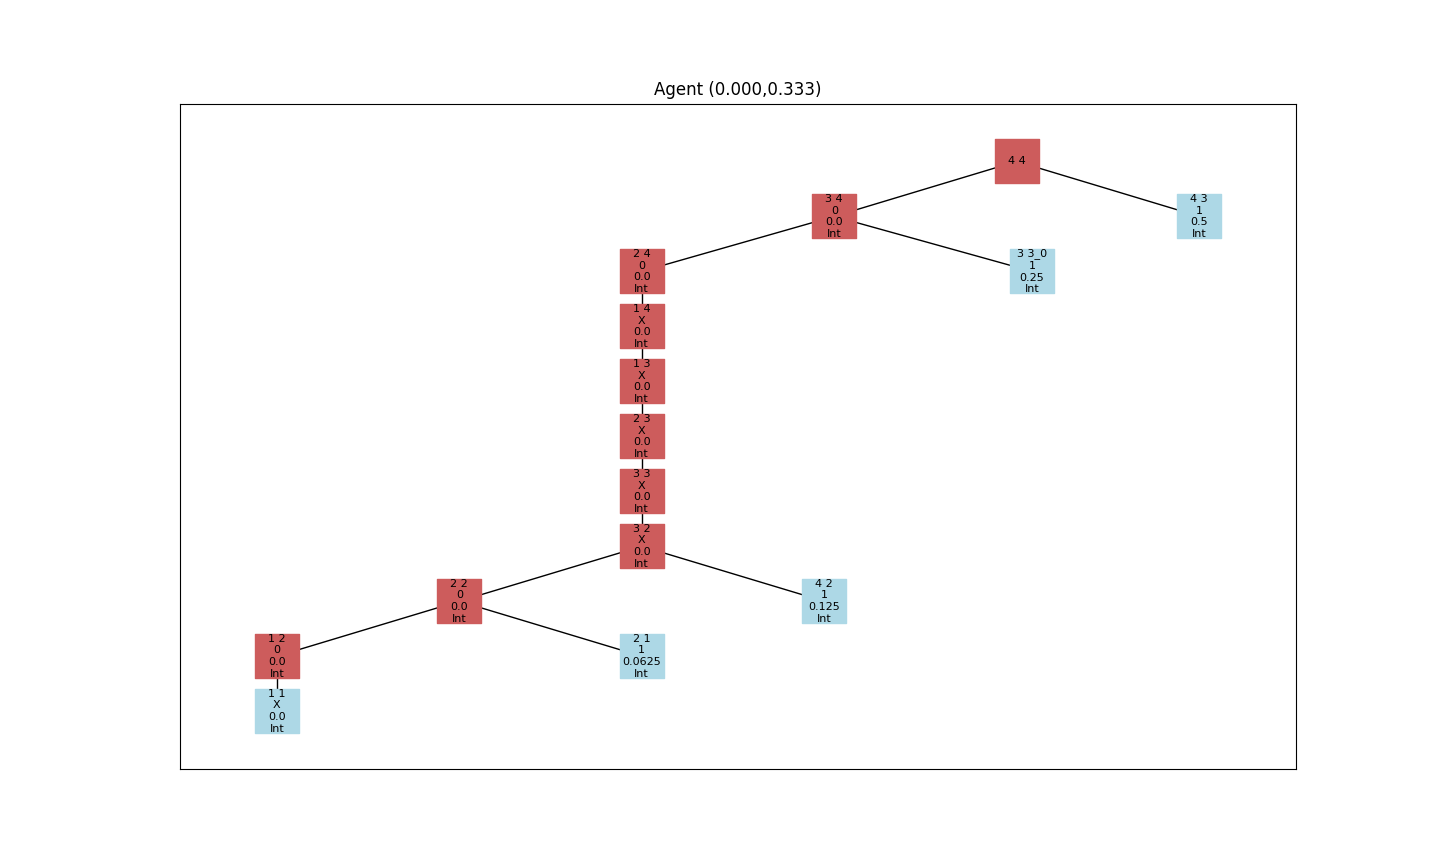
\includegraphics[width=0.40\textwidth]{Cap3/agent_1.png}
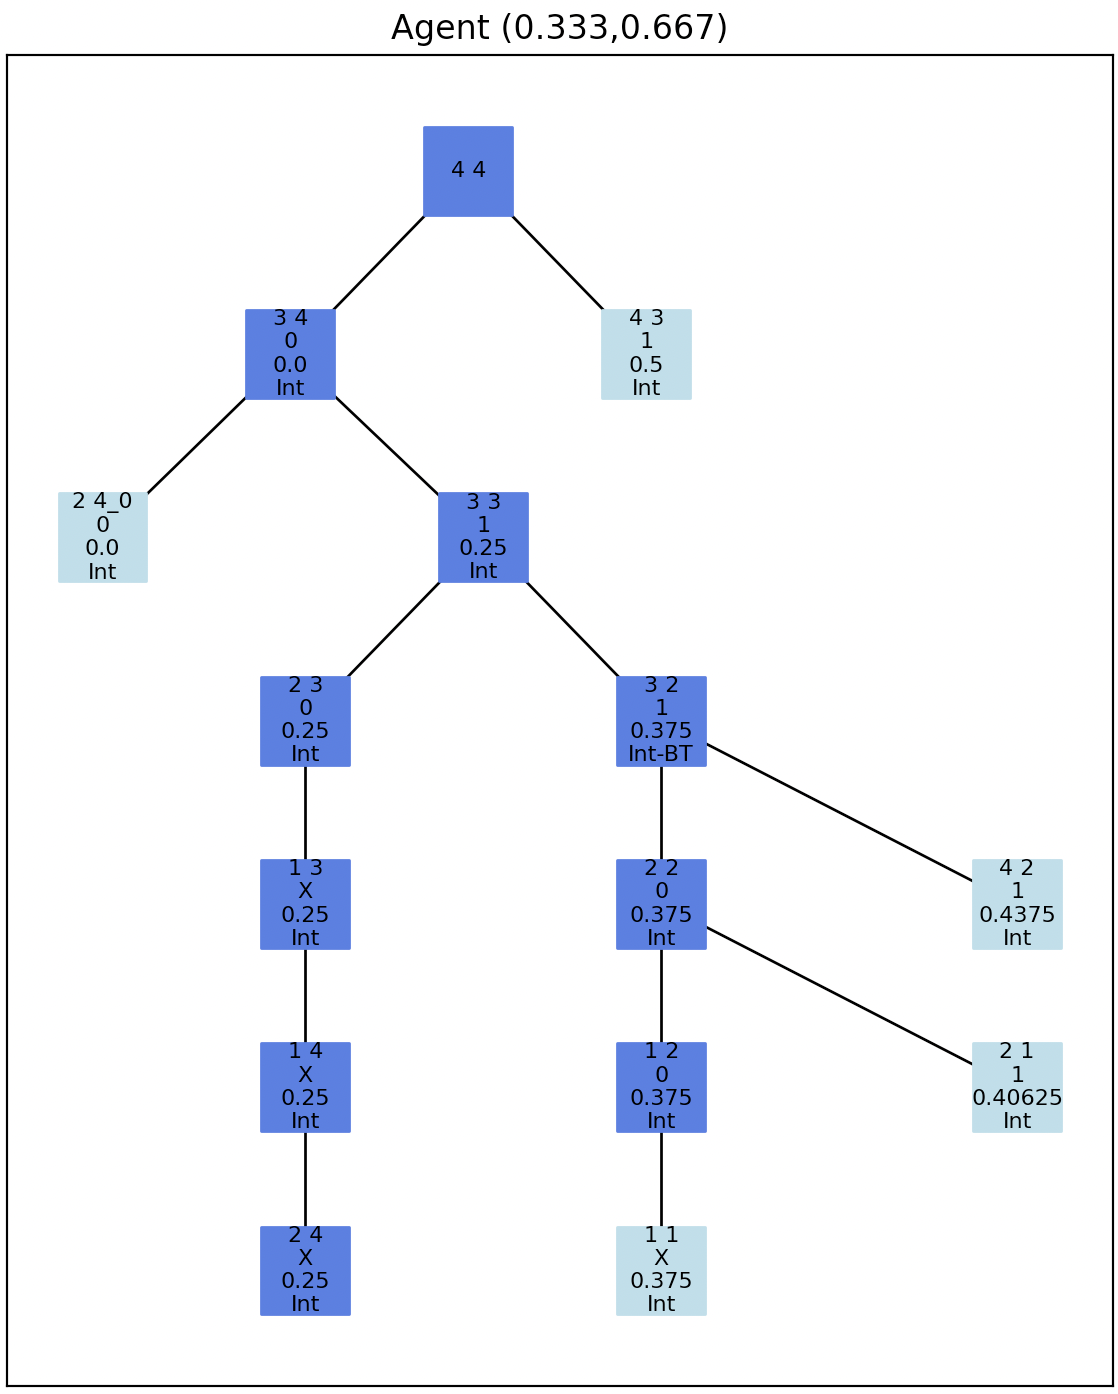
\includegraphics[width=0.40\textwidth]{Cap3/agent_2.png}
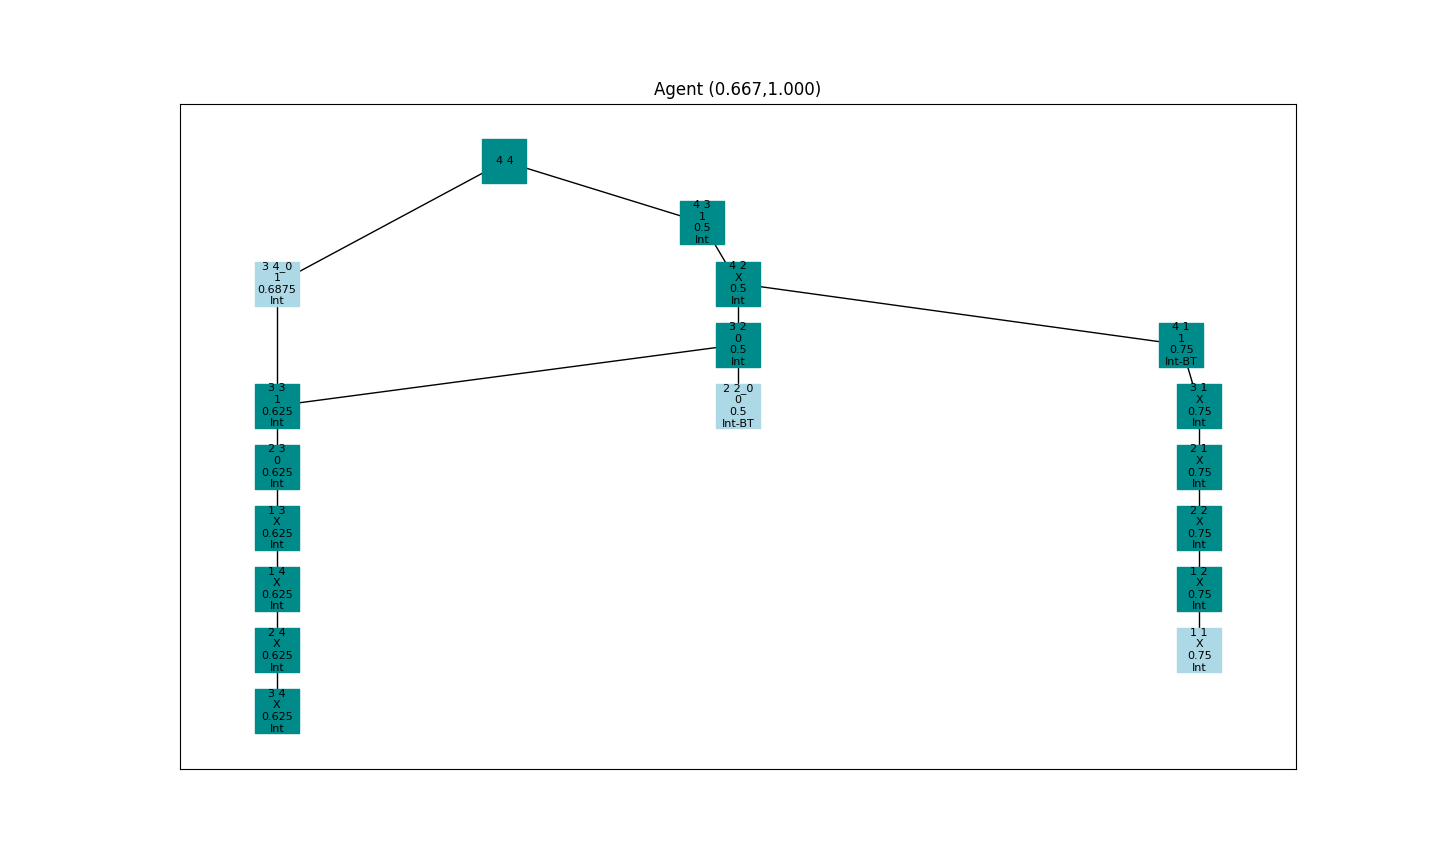
\includegraphics[width=0.40\textwidth]{Cap3/agent_3.png}
\caption{Trees constructed by each agent post-exploration: (a) Agent 1, (b) Agent 2, (c) Agent 3.}
\label{fig_agent_trees}
\end{figure}
    
These visualizations illustrate how each agent independently constructs its own representation of the graph,
adapting to the imperfections and resulting in different exploration paths.
    
    
    
    
    
    